\documentclass[11pt]{article}

\usepackage[a4paper,margin=1in]{geometry}
\usepackage{graphicx}
\usepackage{hyperref}
\usepackage{float}
\usepackage{listings}
\usepackage{xcolor}
\usepackage{tikz}

\usetikzlibrary{arrows.meta, positioning}

\hypersetup{
    colorlinks=true,
    linkcolor=blue,
    urlcolor=blue
}

\title{DnD Campaign Manager API\\
\large COMP3011 Web Services CW1}
\author{Rory Edmonds}
\date{\today}

\begin{document}

\maketitle

\tableofcontents
\newpage


%------------------------------------------------
\section{Introduction}

This report describes the design and implementation of a RESTful web service for managing tabletop role-playing campaigns. The system allows Dungeon Masters to record campaigns, sessions, encounters, and gameplay events while providing analytics derived from recorded events.

The project was implemented using FastAPI, SQLAlchemy, and SQLite. The system follows a layered architecture separating routing logic, database models, repositories, and validation schemas.


%------------------------------------------------
\section{System Overview}

The application provides an API for recording gameplay data and analysing campaign activity.

The system models a tabletop campaign using the following hierarchy:

\begin{center}
Campaign $\rightarrow$ Session $\rightarrow$ Encounter $\rightarrow$ Event
\end{center}

\begin{itemize}
\item \textbf{Campaign}: a long-running narrative managed by a Dungeon Master.
\item \textbf{Session}: a single play session within a campaign.
\item \textbf{Encounter}: a discrete gameplay interaction such as combat.
\item \textbf{Event}: an atomic action such as damage, healing, or spell usage.
\end{itemize}

This hierarchical model enables detailed tracking of gameplay while supporting analytics based on recorded events.


%------------------------------------------------
\section{System Architecture}

The API follows a layered architecture separating concerns across multiple components.

\begin{figure}[H]
\centering
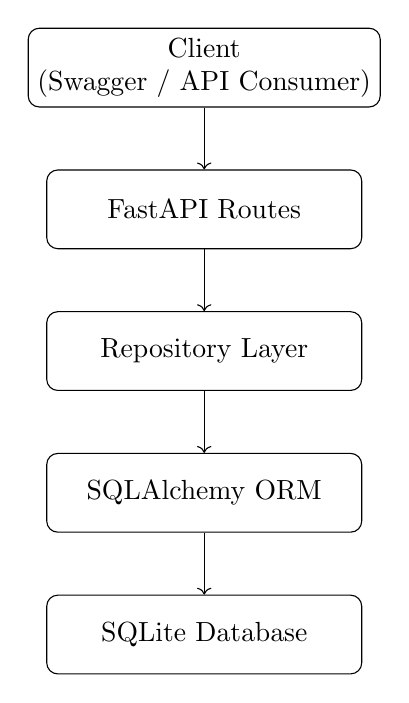
\begin{tikzpicture}[
    node distance=1.8cm,
    box/.style={
        rectangle,
        draw,
        rounded corners,
        minimum width=4cm,
        minimum height=1cm,
        align=center
    }
]

\node[box] (client) {Client\\(Swagger / API Consumer)};
\node[box, below of=client] (routes) {FastAPI Routes};
\node[box, below of=routes] (repos) {Repository Layer};
\node[box, below of=repos] (orm) {SQLAlchemy ORM};
\node[box, below of=orm] (db) {SQLite Database};

\draw[->] (client) -- (routes);
\draw[->] (routes) -- (repos);
\draw[->] (repos) -- (orm);
\draw[->] (orm) -- (db);

\end{tikzpicture}
\caption{System Architecture of the Campaign Manager API}
\end{figure}

The architecture consists of the following layers:

\subsection{API Routes}

Routes define HTTP endpoints using the FastAPI framework. These endpoints validate requests, call repository methods, and return responses.

\subsection{Repositories}

Repositories encapsulate database operations and provide a clean interface between the API layer and the database.

\subsection{Database Models}

SQLAlchemy models define the relational database schema used by the system.

\subsection{Schemas}

Pydantic schemas validate incoming requests and structure outgoing responses.


%------------------------------------------------
\section{Database Design}

The system stores campaign information using a relational schema implemented with SQLAlchemy.

\begin{figure}[H]
\centering
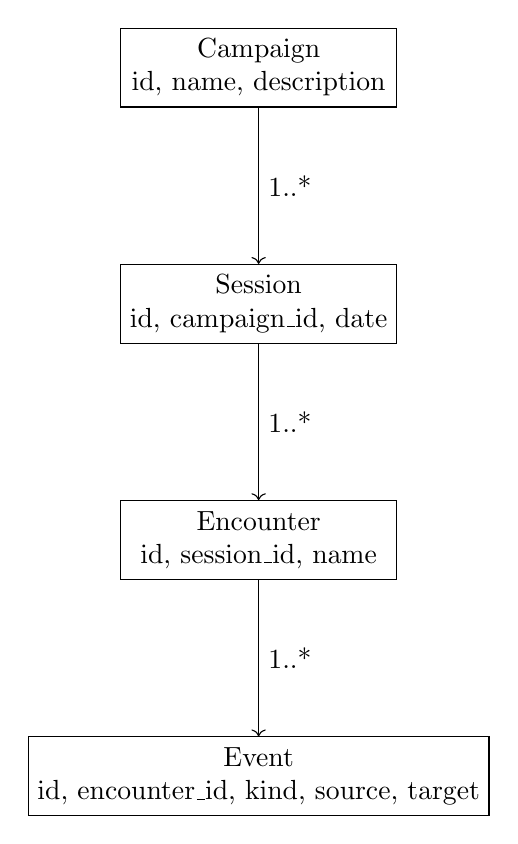
\begin{tikzpicture}[
    node distance=3cm,
    entity/.style={
        rectangle,
        draw,
        minimum width=3.5cm,
        minimum height=1cm,
        align=center
    }
]

\node[entity] (campaign) {Campaign\\id, name, description};

\node[entity, below of=campaign] (session) {Session\\id, campaign\_id, date};

\node[entity, below of=session] (encounter) {Encounter\\id, session\_id, name};

\node[entity, below of=encounter] (event) {Event\\id, encounter\_id, kind, source, target};

\draw[->] (campaign) -- node[right]{1..*} (session);
\draw[->] (session) -- node[right]{1..*} (encounter);
\draw[->] (encounter) -- node[right]{1..*} (event);

\end{tikzpicture}
\caption{Entity Relationship Structure of the Campaign Database}
\end{figure}

The core entities include:

\subsection{Campaign}

Stores high-level campaign information.

\subsection{Session}

Represents a single gameplay session belonging to a campaign.

\subsection{Encounter}

Represents a gameplay interaction such as combat.

\subsection{Event}

Stores atomic gameplay actions such as damage, healing, spell usage, and character status changes.

The event-based design allows complex analytics to be performed by aggregating event data across encounters.


%------------------------------------------------
\section{API Design}

The API follows REST principles and exposes endpoints for managing campaign data.

Example endpoint:

\begin{lstlisting}[language=bash]
GET /api/v1/campaigns
\end{lstlisting}

Core API functionality includes:

\begin{itemize}
\item Campaign CRUD operations
\item Session management
\item Encounter tracking
\item Event logging
\end{itemize}

All endpoints return JSON responses and are documented using OpenAPI.

Interactive documentation is available via FastAPI’s Swagger interface.


%------------------------------------------------
\section{Analytics Features}

The system provides several analytics endpoints derived from recorded events.

\subsection{Damage Leaderboard}

Aggregates total damage dealt by each character across a campaign.

\subsection{Encounter Difficulty Summary}

Summarises encounters based on damage totals and character down events.

\subsection{Event Breakdown}

Counts occurrences of different event types such as damage, healing, and spell usage.


%------------------------------------------------
\section{Testing Strategy}

Automated tests were implemented using \texttt{pytest}.

Tests use FastAPI's TestClient to simulate HTTP requests to the API.

Each test runs against a temporary SQLite database to ensure isolation from development data.

The tests verify:

\begin{itemize}
\item campaign CRUD operations
\item session creation and retrieval
\item encounter management
\item event logging
\item analytics endpoints
\end{itemize}


%------------------------------------------------
\section{Limitations}

Several limitations exist in the current implementation.

\begin{itemize}
\item Event sources and targets are currently stored as text rather than canonical character references.
\item External rule databases for spells and attacks are not yet integrated.
\item Authentication and multi-user support are not implemented.
\end{itemize}


%------------------------------------------------
\section{Future Work}

Future improvements could include:

\begin{itemize}
\item Campaign character registries to avoid event logging inconsistencies.
\item Integration with external DnD spell and monster databases.
\item Authentication and user management.
\item Deployment using containerisation or cloud infrastructure.
\end{itemize}


%------------------------------------------------
\section{Conclusion}

This project demonstrates the design and implementation of a RESTful API for managing tabletop campaign data. The system provides structured storage for campaign activity and enables analytics derived from recorded gameplay events.

The architecture supports extensibility and could be expanded with additional features such as character management and external rules integration.


\end{document}